\documentclass{article}
\usepackage{graphicx}
\usepackage{booktabs}
\usepackage{float}
\usepackage[utf8]{inputenc}
\usepackage[spanish]{babel}
\usepackage{tabularx}
\usepackage{geometry}
\usepackage{afterpage}
\usepackage{array}
\usepackage{colortbl}
\usepackage{xcolor}

\geometry{a4paper, margin=1in}
\newcommand{\separator}{\vspace{5mm}\hrule\vspace{5mm}}

\title{
    \vspace*{3cm}
    \textbf{Proyecto - Entrega 1}\\
    \large Implementación del Juego Mancala
}
\author{
    \text{María Fernanda Rodríguez Ospina} \\
    \small\texttt{mf-rodriguezo@javeriana.edu.co}
    \vspace{3mm}
    \\
    \text{Jeisson Camilo Ruiz Cristancho} \\
    \small\texttt{jeissonc\_ruizc@javeriana.edu.co}
    \vspace{3mm}
    \\
    \text{Alejandro Castelblanco Arias} \\
    \small\texttt{castelblancoa.a@javeriana.edu.co}
    \vspace{1cm}
    \\
    \large Pontificia Universidad Javeriana \\
    \small Facultad de Ingeniería \\
    \small Bogotá, Colombia \\
    \small Abril 2025
}
\date{}

\begin{document}

\maketitle
\thispagestyle{empty}
\clearpage


\pagenumbering{arabic}

\section{Manual de Uso}

\subsection{Preparación del Juego}
\begin{itemize}
    \item \textbf{Tablero}:
    \begin{itemize}
        \item 2 filas (1 por jugador)
        \item 6 pozos (casillas) por fila
        \item 1 almacén (a la derecha de cada fila)
    \end{itemize}
    
    \item \textbf{Semillas Iniciales}:
    \begin{itemize}
        \item 4 semillas en cada pozo
        \item Almacenes vacíos
    \end{itemize}
    
    \item \textbf{Jugadores}:
    \begin{itemize}
        \item Jugador 1: Siempre humano
        \item Jugador 2: Puede ser humano o automático (seleccionado al inicio)
    \end{itemize}
    
    \item \textbf{Turnos}:
    \begin{itemize}
        \item Jugador 1 inicia el juego
    \end{itemize}
\end{itemize}


\subsection{Desarrollo del Juego}
\begin{itemize}
    \item \textbf{Turno de un Jugador}:
    \begin{enumerate}
        \item Elige un pozo (1 al 6) de tu fila que no esté vacío
        \item Recoge todas las semillas de ese pozo
        \item Distribúyelas en sentido antihorario (1 semilla por pozo), saltando el almacén del oponente
    \end{enumerate}
    \item \textbf{Selección de Pozo}:
    \begin{itemize}
        \item \textbf{Humano}: Ingresa un número del 1 al 6 mediante la consola
        \item \textbf{Automático}: Selecciona el pozo con más semillas en la fila del Jugador 2
    \end{itemize}
    \item \textbf{Reglas Especiales}:
    \begin{itemize}
        \item \textbf{Captura}: Si la última semilla cae en un pozo vacío de tu lado, capturas las semillas del pozo opuesto
        \item \textbf{Turno Extra}: Si la última semilla cae en tu almacén, repites turno
    \end{itemize}
\end{itemize}

\subsection{Fin del Juego}
\begin{itemize}
    \item \textbf{Condiciones de Victoria}:
    \begin{itemize}
        \item Cuando un jugador no tiene semillas en sus pozos, el otro recoge las restantes
        \item Gana quien tenga más semillas en su almacén
        \item Empate si ambos tienen la misma cantidad
    \end{itemize}
\end{itemize}

\section{Diagrama de Clases}
\begin{figure}[H]
    \centering
    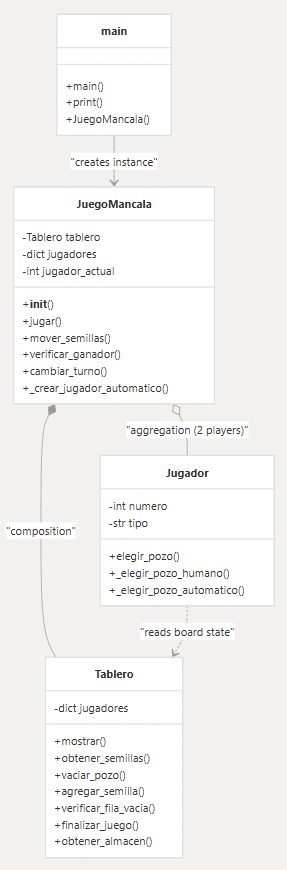
\includegraphics[width=0.5\linewidth]{clases.png} % Ajusta el ancho al ancho de línea
    \caption{Diagrama de clases del juego mancala}
    \label{fig:diagrama}
\end{figure}
El diagrama de clases representa la estructura principal del sistema \textbf{JuegoMancala}, compuesto por tres clases clave: \texttt{JuegoMancala}, \texttt{Tablero} y \texttt{Jugador}. Estas clases colaboran para modelar el funcionamiento del juego Mancala, controlando tanto la lógica de juego como la interacción entre los jugadores y el estado del tablero.

\subsection*{Clase \texttt{JuegoMancala}}

Esta clase centraliza el control del juego. Se encarga de gestionar el flujo de la partida, los turnos, la verificación del estado del juego y la interacción entre jugadores y el tablero.

\begin{itemize}
  \item \textbf{Atributos:}
  \begin{itemize}
    \item \texttt{tablero} : instancia de la clase \texttt{Tablero}.
    \item \texttt{jugador\_actual} : entero que indica el turno actual.
    \item \texttt{jugadores} : mapa de jugadores (\texttt{Map<int, Jugador>}).
  \end{itemize}
  
  \item \textbf{Métodos:}
  \begin{itemize}
    \item \texttt{\_crear\_jugador\_automatico()} : Pregunta si el Jugador 2 será automático o humano
    \item \texttt{mover\_semillas(jugador, pozo)} : Ejecuta la lógica de distribución de semillas
    \item \texttt{verificar\_ganador()} : Determina si hay un ganador
    \item \texttt{cambiar\_turno()} : Cambia al siguiente jugador
    \item \texttt{jugar()} : Determina la lógica general de la partida
  \end{itemize}
\end{itemize}

\subsection*{Clase \texttt{Tablero}}

Representa el estado visual y lógico del tablero. Administra la distribución de semillas, verificación de final de juego y control de almacenes.

\begin{itemize}
  \item \textbf{Atributos:}
  \begin{itemize}
    \item \texttt{jugadores} : mapa donde cada jugador tiene un arreglo de 7 enteros (6 pozos + 1 almacén).
  \end{itemize}
  
  \item \textbf{Métodos:}
  \begin{itemize}
    \item \texttt{mostrar()} : muestra el tablero.
    \item \texttt{obtenerSemillas(jugador, pozo)} : retorna las semillas de un pozo.
    \item \texttt{vaciarPozo(jugador, pozo)} : vacía el pozo indicado.
    \item \texttt{agregarSemilla(jugador, posición)} : añade una semilla a la posición.
    \item \texttt{verificarFilaVacia(jugador)} : comprueba si un jugador ya no tiene semillas.
    \item \texttt{finalizarJuego()} : realiza el conteo final de almacenes.
    \item \texttt{obtenerAlmacen(jugador)} : devuelve la cantidad de semillas del almacén.
  \end{itemize}
\end{itemize}

\subsection*{Clase \texttt{Jugador}}

Modela a cada jugador que participa en el juego.

\begin{itemize}
  \item \textbf{Atributos:}
  \begin{itemize}
    \item \texttt{numero} : identificador del jugador.
    \item \texttt{tipo} : Indica si el jugador es humano o automático

  \end{itemize}
  
  \item \textbf{Métodos:}
  \begin{itemize}
    \item \texttt{elegir\_pozo(tablero)} : Permite seleccionar el pozo desde el cual mover semillas (humano: entrada por consola; automático: elige el pozo con más semillas)
    \item \texttt{\_elegir\_pozo\_humano(tablero)} : Lógica para la selección de pozo por un jugador humano
    \item \texttt{\_elegir\_pozo\_automatico(tablero)} : Lógica para la selección de pozo por un jugador automático
  \end{itemize}
\end{itemize}

\subsection*{Relaciones Entre Clases}

\begin{itemize}
  \item \texttt{JuegoMancala} tiene una relación 1 a 1 con \texttt{Tablero}.
  \item \texttt{JuegoMancala} tiene una relación 1 a muchos con \texttt{Jugador}.
  \item \texttt{Jugador} interactúa con \texttt{Tablero} al elegir pozos.
\end{itemize}

\section{Diagrama de Secuencia}
\begin{figure}[H]
    \centering
    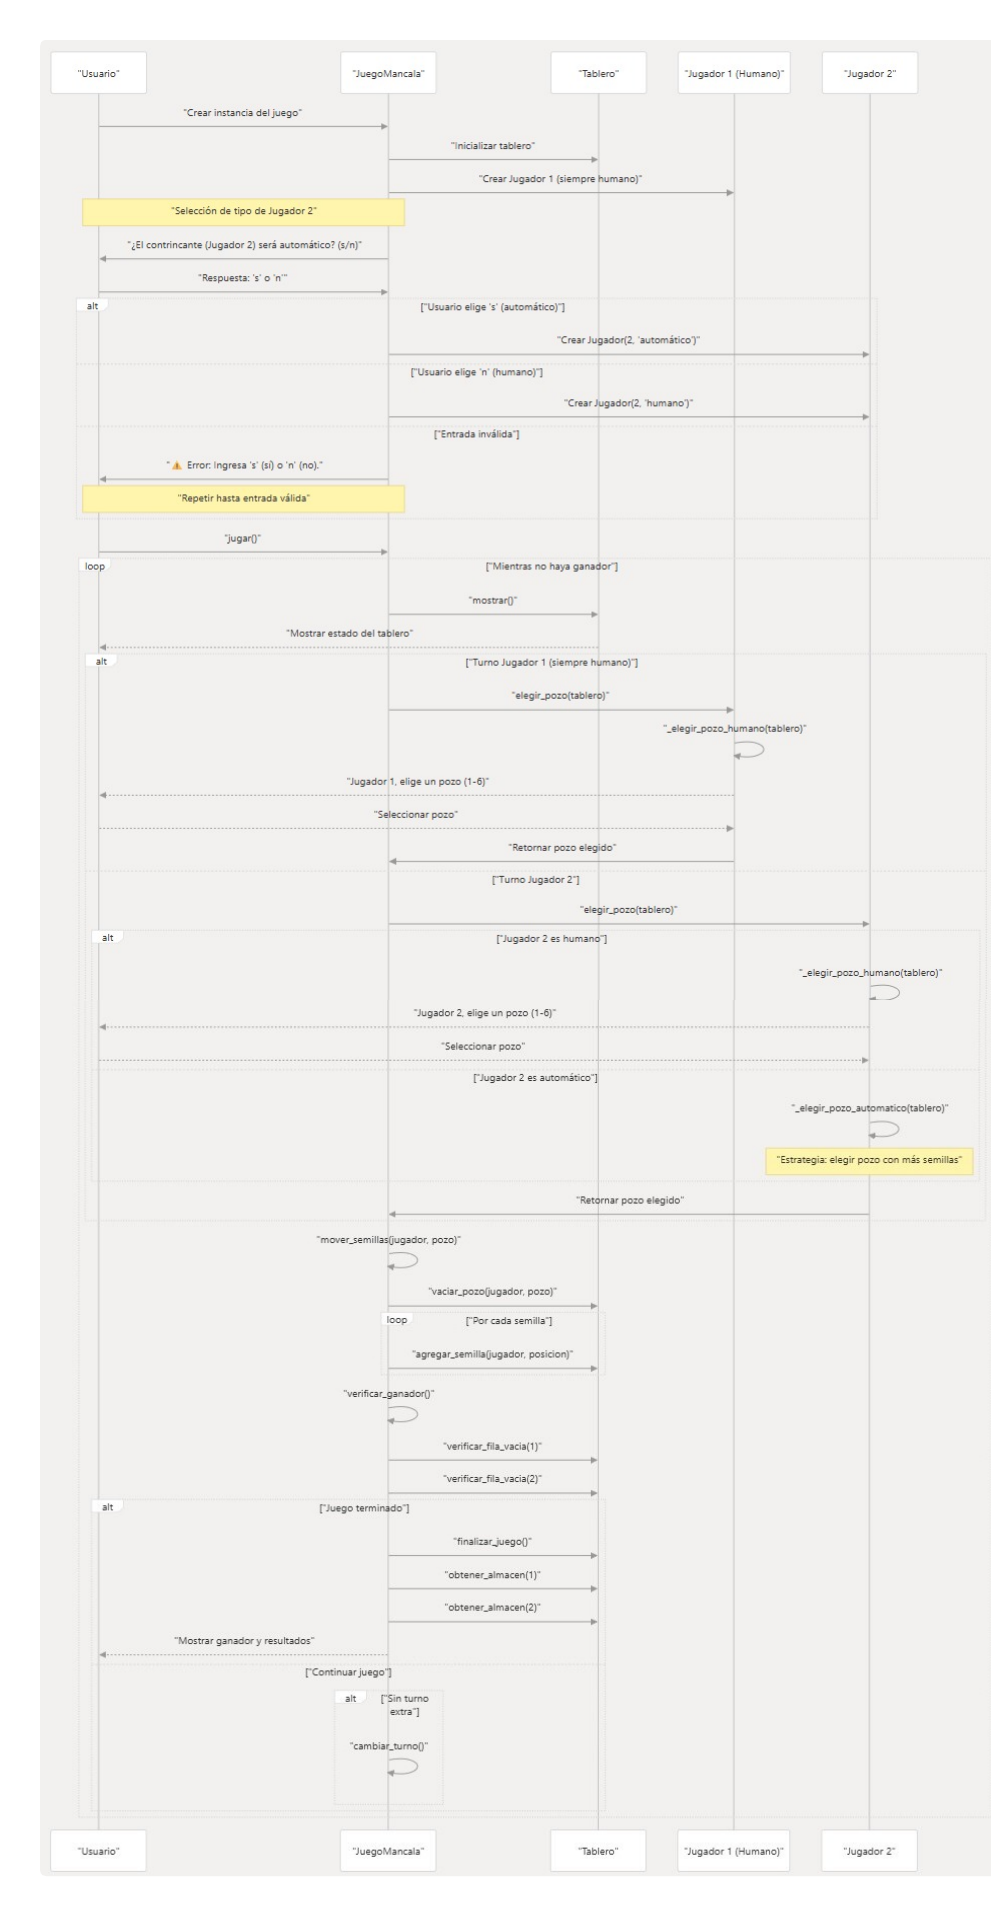
\includegraphics[width=0.8\textwidth]{Diagrama_secuencia.png}
    \caption{Diagrama de secuencia del flujo del juego Mancala}
    \label{fig:diagrama-secuencia}
\end{figure}
El diagrama de secuencia ilustra la interacción entre los diferentes componentes principales del sistema \textbf{JuegoMancala}, incluyendo al \textbf{usuario}, el \textbf{juego}, el \textbf{tablero} y los \textbf{jugadores}.

El flujo comienza con la creación de una instancia del juego por parte del usuario. En ese momento, se inicializan los componentes internos: el tablero y los dos jugadores (Jugador 1 siempre humano, Jugador 2 humano o automático según elección del usuario). Posteriormente, el usuario invoca el método \texttt{jugar()}, el cual inicia un ciclo repetitivo que continúa hasta que se determina un ganador.

Durante cada turno:
\begin{itemize}
    \item El juego muestra el estado actual del tablero
    \item El jugador activo elige un pozo desde el cual mover semillas (humano vía consola, automático seleccionando el pozo con más semillas)
    \item Las semillas se distribuyen en los pozos correspondientes, utilizando el método \texttt{mover\_semillas()}
    \item El sistema verifica si el juego ha terminado usando el método \texttt{verificar\_ganador()}, que consulta al tablero si alguna fila está vacía
    \item Si el juego termina, se muestran los resultados y se determina el ganador en función del contenido de los almacenes
    \item Si el jugador no obtuvo un turno extra, el juego cambia al siguiente jugador
\end{itemize}


Este diagrama permite visualizar claramente cómo se coordinan los mensajes entre clases para ejecutar una partida de Mancala, respetando las reglas del juego y facilitando la interacción entre lógica de negocio, entrada del usuario y estado visual.

\section{Tabla de Requerimientos}
\begin{table}[h]
\centering
\caption{Reglas del Juego Mancala}
\label{tab:reglas}
\begin{tabular}{|>{\centering\arraybackslash}p{3cm}|p{9cm}|}
\hline
\rowcolor[gray]{0.9}
\textbf{Regla} & \textbf{Descripción} \\
\hline
\textbf{Inicialización} & 2 filas × 6 pozos, 4 semillas/pozo, almacenes vacíos. \\ 
\hline
\textbf{Movimiento Válido} & Elegir un pozo no vacío de tu fila (1-6). \\
\hline
\textbf{Distribución} & Antihorario, 1 semilla/pozo, ignorar almacén del oponente. \\
\hline
\textbf{Captura} & Si última semilla cae en pozo vacío propio, capturar pozo opuesto. \\
\hline
\textbf{Turno Extra} & Si última semilla cae en tu almacén, conservas el turno. \\
\hline
\textbf{Fin del Juego} & Cuando un jugador se queda sin semillas. El otro recoge las restantes. \\
\hline
\textbf{Ganador} & Jugador con más semillas en su almacén. \\
\hline
\end{tabular}
\end{table}


\subsection{Ejemplo Visual}

\begin{verbatim}

Turno: Jugador 1
Almacén J1 [0] | Pozos: [4, 4, 4, 4, 4, 4]
Almacén J2 [0] | Pozos: [4, 4, 4, 4, 4, 4]
\end{verbatim}

\subsection{Notas Importantes}
\begin{itemize}
    \item \textbf{Errores Comunes}:
    \begin{itemize}
        \item No elegir pozos vacíos
        \item No distribuir semillas en el almacén del oponente
        \item Olvidar capturar semillas cuando aplica
        \item Visualización repetida del tablero (primero la del movimiento del jugador luego la del jugador automatico)
    \end{itemize}
    \item \textbf{Notas de Implementación}:
    \begin{itemize}
        \item Jugador 1 es siempre humano, con entrada por consola
        \item Jugador 2 puede ser automático, seleccionando el pozo con más semillas
    \end{itemize}
\end{itemize}

\end{document}